\def\year{2019}\relax
%File: formatting-instruction.tex
\documentclass[letterpaper]{article} % DO NOT CHANGE THIS
\usepackage{aaai19}  % DO NOT CHANGE THIS
\usepackage{times}  % DO NOT CHANGE THIS
\usepackage{helvet} % DO NOT CHANGE THIS
\usepackage{courier}  % DO NOT CHANGE THIS
\usepackage[hyphens]{url}  % DO NOT CHANGE THIS
\usepackage{float}
\usepackage{graphicx} % DO NOT CHANGE THIS
\urlstyle{rm} % DO NOT CHANGE THIS
\def\UrlFont{\rm}  % DO NOT CHANGE THIS
\usepackage{graphicx}  % DO NOT CHANGE THIS
\frenchspacing  % DO NOT CHANGE THIS
\setlength{\pdfpagewidth}{8.5in}  % DO NOT CHANGE THIS
\setlength{\pdfpageheight}{11in}  % DO NOT CHANGE THIS
\usepackage{amsmath}
\usepackage{amsthm}


%PDF Info Is REQUIRED.
% For /Author, add all authors within the parentheses, separated by commas. No accents or commands.
% For /Title, add Title in Mixed Case. No accents or commands. Retain the parentheses.
 \pdfinfo{
/Title (Adversarial Examples for Silhouette-based Gait Recognition)
/Author (Cong Lin, ZiJia Chen, Yifan Xu)
} %Leave this	
% /Title ()
% Put your actual complete title (no codes, scripts, shortcuts, or LaTeX commands) within the parentheses in mixed case
% Leave the space between \Title and the beginning parenthesis alone
% /Author ()
% Put your actual complete list of authors (no codes, scripts, shortcuts, or LaTeX commands) within the parentheses in mixed case. 
% Each author should be only by a comma. If the name contains accents, remove them. If there are any LaTeX commands, 
% remove them. 

% DISALLOWED PACKAGES
% \usepackage{authblk} -- This package is specifically forbidden
% \usepackage{balance} -- This package is specifically forbidden
% \usepackage{caption} -- This package is specifically forbidden
% \usepackage{color (if used in text)
% \usepackage{CJK} -- This package is specifically forbidden
% \usepackage{float} -- This package is specifically forbidden
% \usepackage{flushend} -- This package is specifically forbidden
% \usepackage{fontenc} -- This package is specifically forbidden
% \usepackage{fullpage} -- This package is specifically forbidden
% \usepackage{geometry} -- This package is specifically forbidden
% \usepackage{grffile} -- This package is specifically forbidden
% \usepackage{hyperref} -- This package is specifically forbidden
% \usepackage{navigator} -- This package is specifically forbidden
% (or any other package that embeds links such as navigator or hyperref)
% \indentfirst} -- This package is specifically forbidden
% \layout} -- This package is specifically forbidden
% \multicol} -- This package is specifically forbidden
% \nameref} -- This package is specifically forbidden
% \natbib} -- This package is specifically forbidden -- use the following workaround:
% \usepackage{savetrees} -- This package is specifically forbidden
% \usepackage{setspace} -- This package is specifically forbidden
% \usepackage{stfloats} -- This package is specifically forbidden
% \usepackage{tabu} -- This package is specifically forbidden
% \usepackage{titlesec} -- This package is specifically forbidden
% \usepackage{tocbibind} -- This package is specifically forbidden
% \usepackage{ulem} -- This package is specifically forbidden
% \usepackage{wrapfig} -- This package is specifically forbidden
% DISALLOWED COMMANDS
% \nocopyright -- Your paper will not be published if you use this command
% \addtolength -- This command may not be used
% \balance -- This command may not be used
% \baselinestretch -- Your paper will not be published if you use this command
% \clearpage -- No page breaks of any kind may be used for the final version of your paper
% \columnsep -- This command may not be used
% \newpage -- No page breaks of any kind may be used for the final version of your paper
% \pagebreak -- No page breaks of any kind may be used for the final version of your paperr
% \pagestyle -- This command may not be used
% \tiny -- This is not an acceptable font size.
% \vspace{- -- No negative value may be used in proximity of a caption, figure, table, section, subsection, subsubsection, or reference
% \vskip{- -- No negative value may be used to alter spacing above or below a caption, figure, table, section, subsection, subsubsection, or reference

\setcounter{secnumdepth}{0} %May be changed to 1 or 2 if section numbers are desired.

% The file aaai19.sty is the style file for AAAI Press 
% proceedings, working notes, and technical reports.
%
\setlength\titlebox{1.75in} % If your paper contains an overfull \vbox too high warning at the beginning of the document, use this
% command to correct it. You may not alter the value below 2.5 in
\title{Adversarial Examples for Silhouette-based Gait Recognition Networks}
%Your title must be in mixed case, not sentence case. 
% That means all verbs (including short verbs like be, is, using,and go), 
% nouns, adverbs, adjectives should be capitalized, including both words in hyphenated terms, while
% articles, conjunctions, and prepositions are lower case unless they
% directly follow a colon or long dash
\author{\\Cong Lin,\quad ZiJia Chen,\quad Yifan Xu\\  \texttt{\{cl3954,zc2521,yx2502\}@columbia.edu}}


\makeatletter
\def\@copyrightspace{\relax}
\makeatother

\begin{document}


\maketitle

\begin{abstract}
The development of deep neural networks for gait recognition in recent years provides a new approach to building gait recognition security systems. However, it has been demonstrated that deep neural networks are vulnerable to adversarial example attacks, which will jeopardize the whole security system. In this paper, we particularly study and design adversarial examples against silhouette-based gait recognition neural networks typical of models in the research field. By adopting Fast Gradient Sign Method, we produce imperceptible perturbation added to the source silhouette frames or gait energy images and cause the neural network to return the target prediction. We also try to combine adversarial example methods for attacking segmentation neural networks so as to break down the entire gait recognition security system. We carry out experiments on several models and the widely used gait dataset CASIA, with current results justifying the practicability of our methods.

\end{abstract}

\subsection{1. Introduction}
Gait recognition has been frequently recognized as a step beyond facial recognition. Models for this task are being built in multiple crucial safety fields such as recognizing criminals from a footage video, identifying people that looks similar in airport security, etc. In the past few years, with the fast development of deep learning, deep neural network models have been introduced to gait recognition, resulting in many novel gait recognition frameworks. Due to the powerful expressiveness of neural networks, performance in gait recognition tasks has been pushed to a new higher level, which is a guarantee for the reliability of neural-network-based gait recognition security systems.

Among different types of gait recognition neural network models, models that take silhouette frames or the deduced averaged gait energy images (GEI) as inputs are very common, and in this paper we refer to them as silhouette-based gait recognition network. Silhouette frames are cropped frames of gait record video in which figure of the person being recorded is labeled in white while the background in black. They are basically genenrated using image segmentation models. By averaging a number of consecutive silhouette frames, we can get the gait energy image which describes the cumulative spatial distribution of the person's movement. Take the silhouette frames or GEI as input, silhouette-based gait recognition networks extract latent features underneath, and return the corresponding feature vector. In convention, the feature vector will be compared with those in the database in metrics like Euclidean distance for estimating identity. By elaborating objective function in the training phase, the recognition network can learn to generate feature vectors that are sufficient for identifying and distinguishing people, which is promising for applications in practice.

However, despite their performance and unprecedented progress made in a variety of fields, neural networks are justified to be lack of robustness under the attack of adversarial examples. That is, there exist some slightly modified source inputs that can cause the neural network to incorrect outputs or even any desired outputs. This indicates that, in the case of gait recognition, we can generate adversarial silhouette frame examples or adversarial GEI examples to hack a neural-network-based gait recognition security system. If this is practicable, then it will be a devastating flaw in such security system.

The key points in this adversarial example attack task are that: 1) the adversarial example should be indstinguishable from the original image for human eyes, namely making the perturbation imperceptible, 2) the adversarial example is not restricted to only be generated for a single image, but rather for a sequence of frame images, 3) in order to hack the entire system, the adversarial example in real-life source video level needs to fool both the segmentation network and the gait recognition network, which can be two non-end-to-end models.

In this paper, we focus on these problems and study the adversarial examples against gait recognition networks. To achieve the final target of generating real-life adversarial gait record video examples, we divide the task into the following parts and tackle them one by one: 
\begin{figure*}[t]
\centering
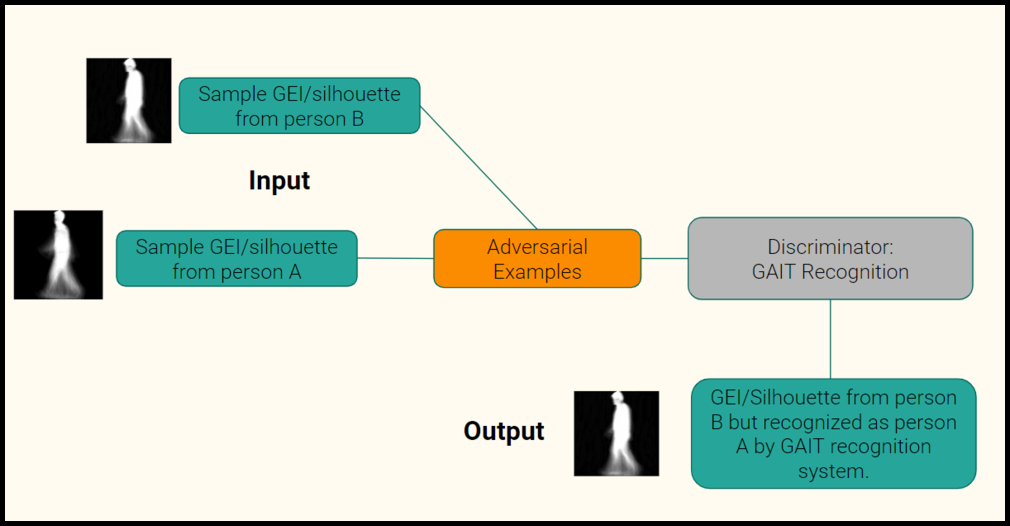
\includegraphics[width=0.8\textwidth]{dl4.png} 
\caption{Adversarial Examples to GAIT Recognition Algorithm}
\label{fig2}
\end{figure*}
\begin{itemize}
\item Based on the silhouette frames or the derived GEI of a source person and that of a target person, generate an adversarial example for the source person in which he will be identified as the target person by the neural network.

\item Based on a static background picture and the silhouette frames or the derived GEI of a target person, generate an adversarial example in which the target person will be detected by the neural network.

\item Based on a gait record video of a source person and the silhouette frames or the derived GEI of a target person, generate an adversarial example for the source person in which he will be identified as the target person by the neural network.
\end{itemize}

Our algorithm for generating adversarial examples mainly based on Fast Grandient Sign Method (FGSM) and methods for generating adversarial examples against segmentation networks.

To sum up, our contributions in this paper are listed below:

\begin{itemize}
\item We point out the danger of adversarial examples to neural-network-based gait recognition security system.

\item We generate adversarial examples against several silhouette-based gait recognition networks.

\item We devise an algorithm for generating adversarial examples against non-end-to-end models.
\end{itemize}

\subsection{2. Related Works}

\subsubsection{2.1. Gait Recognition Networks}
The cross-view gait methods can be categorized into three types: features-invariant model, 3D construction model, and View Transformation Model (VTM). [10] proposed an updated feature selection solution which reduced misclassification for the view-invariant gait recognition problem. [11] proposed an arbitrary view gait recognition method where the gait recognition is performed in 3D to be robust to variation in speed, inclined plane and clothing, and in the presence of a carried item. The most prevailing one now is View Transformation Model which can project a large, dimensional, multi-view gait data into a lower-dimensional feature space such as silhouette and GEI image (Gait energy image)that has sufficient discriminative capability. [4] developed a specialized deep CNN architecture for Gait Recognition which is less sensitive to several case of common variations and occlusions that affect and degrade gait recognition performance. 

\subsubsection{2.2. General Adversarial Examples}
Generating adversarial examples for classification has been extensively studied. In [7], Adversarial examples were broadly discussed. An adversarial example is a sample of input data which has been modified very slightly in a way that is intended to cause a machine learning classifier to misclassify it. In many cases, these modifications can be so subtle that a human observer can not notice it at all, yet the machine learning classifier still makes a mistake. [7] majorly demonstrated how to feed adversarial images obtained from a cell-phone camera to an ImageNet Inception classifier and measure the classification accuracy of the system. [8] proposed a simple and fast yet more accurate gradient sign method to generate adversarial examples based on the linear nature of CNN.[9] efficiently trained feed-forward neural networks in a self-supervised manner to generate adversarial examples for a particular target model or a particular set of networks.

\subsubsection{2.3 Adversarial Examples for Semantic Segmentation and Object Detection}
[1] proposed an algorithm named Dense Adversary Generation (DAG) to generate a large family of adversarial examples and apply them to a wide range of deep networks for segmentation and detection. [1] elaborated a possibility of adversarial perturbations being transferred across networks with different training data, based on different architectures, and even for different recognition tasks. [2] proposed a way of how existing adversarial attackers can be transferred to the task of semantic segmentation and possibility of creating imperceptible adversarial perturbations that lead a deep network to misclassify almost all pixels of a chosen class while leaving network prediction nearly unchanged outside of that class.

 \begin{figure}
\centering
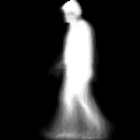
\includegraphics[width=0.6\columnwidth]{dl1.png} 
\caption{GEI Image from person B}
\label{fig2}
\end{figure}

 \begin{figure}
\centering
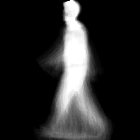
\includegraphics[width=0.6\columnwidth]{dl2.png} 
\caption{GEI Image from person A}
\label{fig3}
\end{figure}

 \begin{figure}
\centering
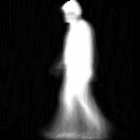
\includegraphics[width=0.6\columnwidth]{dl3.png} 
\caption{GEI Image from person B but considered to be person A by gait recognition system}
\label{fig4}
\end{figure}
\bigskip
 \begin{figure}
\centering
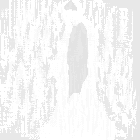
\includegraphics[width=0.6\columnwidth]{dlnoise.png} 
\caption{Noise we added to person B GEI image}
\label{fig5}
\end{figure}
\subsubsection{2.4 Adversarial Examples on Gait Recognition system}
There aren’t none prior experiment on Adversarial Examples to Gait Recognition system before. [12] proposed the vulnerability of the motion sensor-based gait authentication algorithm with adversarial perturbations, obtained via the simple fast-gradient sign method.. However, it’s mainly focusing on mainly sensor-based Gait mechanism which has been tackled long while ago. [13] proposed a spoof attack on sensor-based gait authentication system on 2007 and it demonstrated that, in sensor based gait recognition,  attackers with knowledge of their closest person in the database can be a serious threat to the authentication system. On the contrary, within this article, we will be focusing on silhouette based gait recognition system with segmentation which claimed to be more advanced and accurate.


\subsection{3. Methods}
Most silhouette-based gait recognition networks tranform the raw input into feature vector and compare feature vectors in terms of distance or similarity metrics to predict the person identity. If we denote $x_1,...x_n$ the raw input, $f$ the gait recognition network, $g$ the distance loss function, $x$ a query input and $\hat{y} \in \{1,...n\}$ is the corresponding predicted identity, then the procedure of the gait recognition network system can be summarized as:
$$\hat{y}=arg\min_{i}g(f(x),f(x_i)).$$
Since neural networks are trained using backpropagation and are thereby differentiable, a practicable to generate adversarial example based on a raw input is to fix the network and use a objective function and backpropagation to update the raw input. A typical iterative method is the Fast Gradient Sign Method (FGSM) [8] which can be formulated as 
$$\eta = \epsilon\cdot sgn(\nabla_{x}J(\theta,x,f(x))),$$
where $\eta$ is the update to the current $x$, $\epsilon$ is the step and $J$ is a loss function taking $\theta$ as parameters.

To our concern, given a source image $x$, a target $x'$ and a gait recognition network $f_{\theta}$, we are to generate an adversarial exmaple $x+r$ such that $||f_{\theta}(x+r)-f_{\theta}(x')||_2$ is minimized while $||r||_\infty$ is small. To achieve this, we use algorithm based on FGSM and $L_\infty$ norm constrain:
\begin{equation*}
\left\{
\begin{array}{lr}
r_{t+1}= r_t - \epsilon\cdot sgn(\nabla_{r_t}(||f(x+r_t)-f(x')||_2))\\
\text{clip } \text{elements of } r_{t+1} \text{ within } [-\eta,\eta]\\
t = t + 1\\ 
\end{array}
\right.
.
\end{equation*}
In each iteration, we first adopt FGSM to update the $r$ on $x$, but this may cause too much modification as iterations go on. To address this issue, a clip operation is taken right after FGSM which ensure that the $L_\infty$ norm of $r$ is not larger than a given threshold $\eta$.



\subsection{4. Experiments}

We carry experiments on GaitCNN modified from [4]: A convolutional Neural Network for gait Recognition and CASIA-B: A large multiview gait database. Three variations, namely view angle, clothing and carrying condition changes, are separately considered. We have already conducted two experiments on normal walking datasets without carrying object from view angle of 90 degree, which is the datasets used on mostly gait recognition system. We firstly trained the GaitCNN which can reach up to accuracy of 95\% on test dataset. Then we used FGSM with the learning rate of 0.001 to train the r to change the origin image to be detected as target image by the above gait recognition system. Also, we set a threshold value of 5 unit per pixel to let the r not perturb origin image more than 5 unit per pixel, which can prevent the changes from being detected by human.

\subsection{5. Results}
From the result of experiments above, the result image: the source image, target image, fake image and added noise are in Figure 6; following the evaluation criteria of [14],  we also evaluate the origin image accuracy, fake image accuracy and $l_2$ distance between the origin image and fake image, the result are in Figure 7:
\begin{figure}
\centering

Source Image:

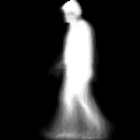
\includegraphics[width=0.3\columnwidth]{dl1.png}
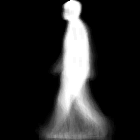
\includegraphics[width=0.3\columnwidth]{ex2-source.png}

Target Image:

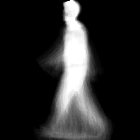
\includegraphics[width=0.3\columnwidth]{dl2.png}
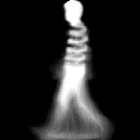
\includegraphics[width=0.3\columnwidth]{ex2-target.png}

Fake Image:

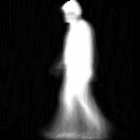
\includegraphics[width=0.3\columnwidth]{dl3.png}
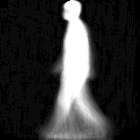
\includegraphics[width=0.3\columnwidth]{ex2-fake.png}

Added Noise:

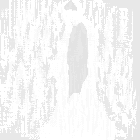
\includegraphics[width=0.3\columnwidth]{dlnoise.png}
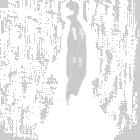
\includegraphics[width=0.3\columnwidth]{ex2-noise.png}

\caption{Result Image}
\label{fig2}
\end{figure}

\begin{figure}[htbp]
\centering
\caption{Evaluation}
\label{vtable}
\begin{tabular}{c|c|c|c}
\hline
$experiment$ & $Accuracy_{origin}$ & $Accuracy_{attack}$ & $l_2 distance$ \\
\hline
1 & 100\% & 0\% & 3.062  \\
2 & 90\% & 0\% & 1.858 \\
Average & 95\% & 0\% & 2.46\\ 
\hline
\end{tabular}
\end{figure}


\subsection{6.References}
\smallskip \noindent
[1] Xie, Cihang, et al. \textit{"Adversarial examples for semantic segmentation and object detection."} Proceedings of the IEEE International Conference on Computer Vision. 2017.

\smallskip \noindent
[2] Fischer, Volker, et al. \textit{"Adversarial examples for semantic image segmentation."} arXiv preprint arXiv:1703.01101 (2017).

\smallskip \noindent
[3] Shiraga, Kohei, et al. \textit{"GEINet: View-invariant gait recognition using a convolutional neural network."} 2016 international conference on biometrics (ICB). IEEE, 2016.

\smallskip \noindent
[4] Alotaibi, Munif, and Ausif Mahmood. \textit{"Improved gait recognition based on specialized deep convolutional neural network."}  Computer Vision and Image Understanding 164 (2017): 103-110.

\smallskip \noindent
[5] Zhang, Cheng, et al. \textit{"Siamese neural network based gait recognition for human identification."} 2016 IEEE International Conference on Acoustics, Speech and Signal Processing (ICASSP). IEEE, 2016.

\smallskip \noindent
[6] Feng, Yang, Yuncheng Li, and Jiebo Luo. \textit{"Learning effective gait features using LSTM."} 2016 23rd International Conference on Pattern Recognition (ICPR). IEEE, 2016.

\smallskip \noindent
[7] Akhtar, Naveed, and Ajmal Mian. "Threat of adversarial attacks on deep learning in computer vision: A survey." IEEE Access 6 (2018): 14410-14430.

\smallskip \noindent
[8] I. J. Goodfellow, J. Shlens, and C. Szegedy. Explaining and harnessing adversarial examples. InICLR, 2015.

\smallskip \noindent
[9] S. Baluja and I. Fischer. Adversarial transformation net-works: Learning to generate adversarial examples. arXiv preprint arXiv:1703.09387, 2017.

\smallskip \noindent
[10] Jia, Ning et al. “On view-invariant gait recognition: a feature selection solution.” IET Biometrics 7 (2018): 287-295.

\smallskip \noindent
[11] Luo, Jian et al. “Robust arbitrary view gait recognition based on parametric 3D human body reconstruction and virtual posture synthesis.” Pattern Recognition 60 (2016): 361-377.

\smallskip \noindent[12]V. U. Prabhu and J. Whaley. Vulnerability of deep learning-
based gait biometric recognition to adversarial perturbations.
In CVPR Workshop on The Bright and Dark Sides of Com-
puter Vision: Challenges and Opportunities for Privacy and
Security (CV-COPS 2017), 2017. 2

\smallskip \noindent [13]Davrondzhon Gafurov, Einar Snekkenes, and Patrick Bours. Spoof attacks on gait
authentication system. IEEE Transactions on Information Forensics and Security,
2(3), 2007. Special Issue on Human Detection and Recognition.

\smallskip \noindent [14] Athalye A, Engstrom L, Ilyas A, et al. Synthesizing robust adversarial examples[J]. arXiv preprint arXiv:1707.07397, 2017.


\end{document}
